% !TeX root = ../main.tex
% -*- coding: utf-8 -*-

\chapter{基于近边界数据的模型所有权推断方法分析}\label{5}

本文选择在开源数据集CIFAR-10\cite{krizhevsky2009learning},Heritage\cite{Heritage},Intel\_image\cite{Intel_image}上进行实验,并选择ResNet18作为评估的源模型,VGG11作为对照的无关模型。本章将从生成初始近边界数据的方法选择,数据近边界特性评估,微调目标分类边界的影响,推断模型所有权的有效性和不同规模近边界数据的可伸缩性扩展这几个方面对本文提出的方法进行测评和分析。

\noindent\textbf{被盗模型:}本文设置了几种常见的模型盗窃方法,包括模型微调,模型剪枝(不同的剪枝率)和模型知识蒸馏,并在源模型的基础上派生得到被盗模型。

\section{实验设置}\label{5.1}

\subsection{数据集}

\noindent\textbf{CIFAR-10:}CIFAR-10共有10个类别,其中训练集包含50000张大小为32x32的图像,测试集包含10000张大小为32x32的图像。

\noindent\textbf{Heritage:}Heritage共有10个类别,其中训练集包含10235张大小为128x128的图像,测试集包含1404张大小为64x64的图像。

\noindent\textbf{Intel\_image:}Intel\_image共有6个类别,其中训练集包含14034张大小为150x150的图像,测试集包含3001张大小为150x150的图像。

\subsection{目标模型}

本文的目标模型选用ResNet18,在上述三个数据集上分别训练作为实验源模型,使用VGG11作为无关的对照模型。ResNet18和VGG11的参数信息如表\ref{table:10}所示。由于CIFAR-10的图片尺寸较小,所以训练的时候将原始ResNet18中首层使用的7x7卷积核改成3x3,步长和填充随之改为1,并且舍弃最大池化层,更改结构后ResNet18在CIFAR-10上的预测准确度得到了提升。

\begin{table}[H]
	\centering
%	\setlength{\arrayrulewidth}{0.5mm}
	\renewcommand\arraystretch{1.2}
	\caption{模型参数信息}
	\label{table:10}
	\begin{tabular*}{13cm}{@{\extracolsep{\fill}} l c c c }
		
		\hline
		模型      &   层数    &   计算量/亿     &    参数量/百万     \\
		\hline

        ResNet18  &   18     &    9.559     &    11.670     \\

		VGG11     &   11     &    47.022    &    132.863     \\

		\hline		
	\end{tabular*}
\end{table}

\subsection{实验环境和参数设置}

本文在实验中的使用的硬件与软件配置如表\ref{table:11}所示。

\begin{table}[H]
	\centering
%	\setlength{\arrayrulewidth}{0.5mm}
	\renewcommand\arraystretch{1.2}
	\caption{硬件与软件配置}
	\label{table:11}
	\begin{tabular*}{13cm}{@{\extracolsep{\fill}} l c }
		
		\hline
		硬件/软件      &   版本    \\
		\hline
		
		操作系统  &   Ubuntu 20.04 LTS    \\
		
		CPU     &   Intel Core i7-11700KF @ 3.6GHz       \\
		
		显卡     &   NVIDIA GeForce RTX 3080 Ti \\
		
		CUDA版本     &   	11.6          \\
		
		机器学习框架     &   pytorch 1.9.0          \\
		
		Python     &   3.7.11           \\
		
		\hline		
	\end{tabular*}
\end{table}

训练过程中Adam优化器并将学习率(Learning rate),迭代轮次(Epoch)和每批次大小(Batch size)分别设置为0.0001,200和64。蒸馏模型实验选择从Resnet18蒸馏至VGG11,蒸馏时将蒸馏温度设置为20并且教师模型比例$\alpha$=0.7,训练轮次是20。初始近边界数据生成采用$CW$-$L_2$算法,实验中选择有目标的生成方式,且学习率,迭代次数和二分搜索次数分别设置为0.001,1000和6,其他参数为默认值。私有近边界数据生成器采用DCGAN的基础结构,训练过程使用Adam优化器且将学习率,训练轮次和每批次大小分别设置为0.0002,8000和64。本方法最后微调源模型阶段需要交替使用源模型损失函数和微调目标边界的损失函数来微调源模型,具体设置为10个轮次交替一次且交替次数最多为10次。



\section{生成初始近边界数据的算法选择}\label{5.2}

本小节将对\ref{3}\ref{3.2}中提到的FGSM,IGSM,RFGSM和CW-$L_2$进行测试,除对CW-$L_2$进行了改进外,其余均使用原作者发布的实现。FGSM,IGSM,RFGSM中均有一个用于界定噪声$\epsilon$的参数。我们进行大量的实验探索选择合适的参数用于与CW-$L_2$进行比较。此外,CW-$L_2$的实验设置如\ref{5.1}所示。

\begin{table}[H]
	\centering
%	\setlength{\arrayrulewidth}{0.5mm}
	\renewcommand\arraystretch{1.2}
	\caption{不同算法生成样本到分类边界的平均距离}
	\label{table:1}
	\begin{tabular*}{13cm}{@{\extracolsep{\fill}} l c c c c}
		
		\hline
		数据集                    &   FGSM   &   IGSM   &  RFGSM  &   CW-$L_2$    \\
		\hline
\multirow{3}{6em}{CIFAR-10}      &    0.557  &   0.430  &  0.418   &    0.066     \\
		                         &    0.461  &   0.419  &  0.373   &    0.103     \\
		                         &    0.586  &   0.369  &  0.356   &    0.112     \\
		\hline
\multirow{3}{6em}{Heritage}      &    0.347  &   0.356  &  0.314   &    0.014     \\
		                         &    0.377  &   0.340  &  0.281   &    0.016     \\
		                         &    0.348  &   0.332  &  0.276   &    0.010     \\
		\hline
\multirow{3}{6em}{Intel\_image}  &    0.522  &   0.447  &  0.353   &    0.088     \\
		                         &    0.475  &   0.506  &  0.387   &    0.122     \\
		                         &    0.468  &   0.402  &  0.428   &    0.127     \\
		\hline		
	\end{tabular*}
\end{table}

FGSM,IGSM,RFGSM和CW-$L_2$到分类边界的距离如表\ref{table:1}所示。从表中可以看出FGSM的效果较差,这是因为FGSM生成对抗性样本只进行一次噪声的添加,效率非常高,在追求效率的情况下牺牲了性能,这是合理的。相比于FGSM,IGSM和RFGSM的效果稍好,这是在算法中引入迭代的效果,通过每次一小步的迭代,不断地在上一次的基础上添加噪声,使得图片以更小的幅度变化。这和表\ref{table:1}中大部分情况下,IGSM和RFGSM的生成的对抗性样本距离分类边界的平均距离比FGSM生成的近是相符的。改进过的CW-$L_2$是这几种方法中效果相当显著,距离分类边界的距离比其他三种方法小数十倍。这是因为本身这个算法机制比较复杂,在迭代的过程中引入了二分查找和神经网络来训练参数以更好的生成图片,我们进一步在算法中引入了到分类边界距离这个参数,使得生成图片朝着距离更小的方向改进,并且达到我们预定的阈值$\theta$时,提前终止算法,一定情况下缓解该算法效率低下的问题。


\section{数据近边界特性的评估}\label{5.3}

本文提出的近边界数据不仅在源模型在表现出了近边界性,在所有盗窃模型中也表现出了这个特点,数据近边界特性的可转移性,是本文提出方法的重要基础。本节将在三个数据集和不同分类边界上对近边界数据的近边界性和可转移性进行测评。

\begin{figure}[!htb]
	\centering
%	\setlength{\abovecaptionskip}{0mm}
%		\vspace{-3mm}
%	\setlength{\belowcaptionskip}{-4mm} %调整图片标题与下文距离
	\subfigure{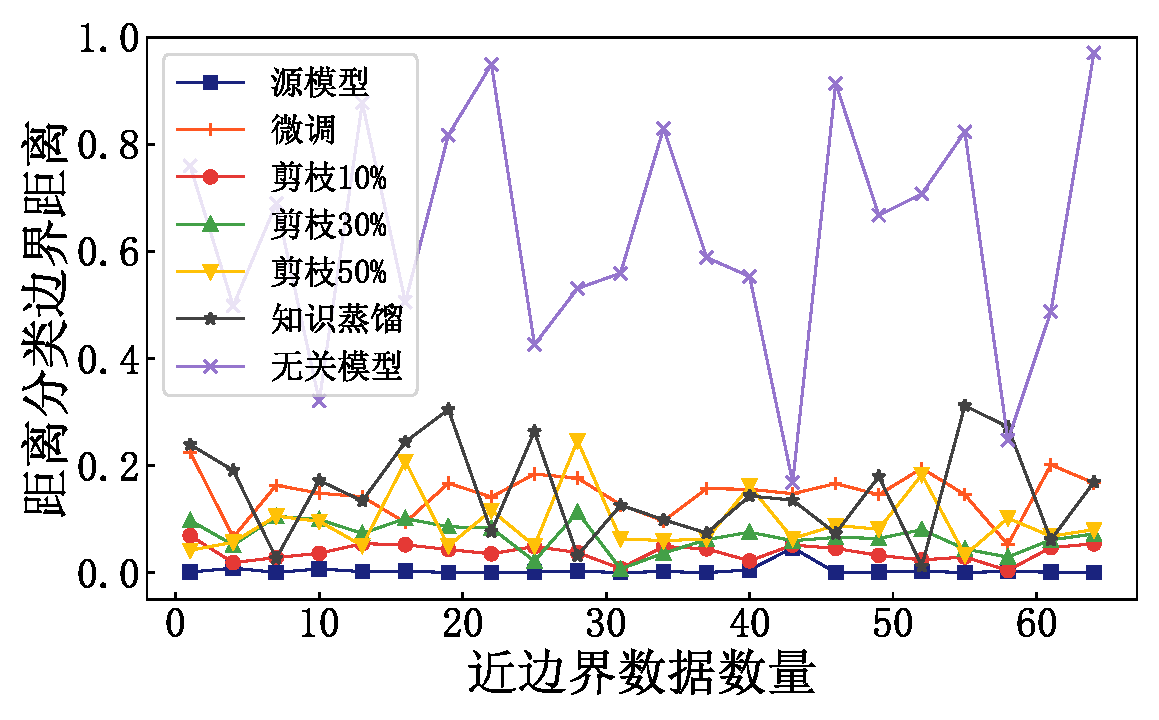
\includegraphics[width=0.49\linewidth]{CIFAR-10-4-2-distance.pdf}} 
	\subfigure{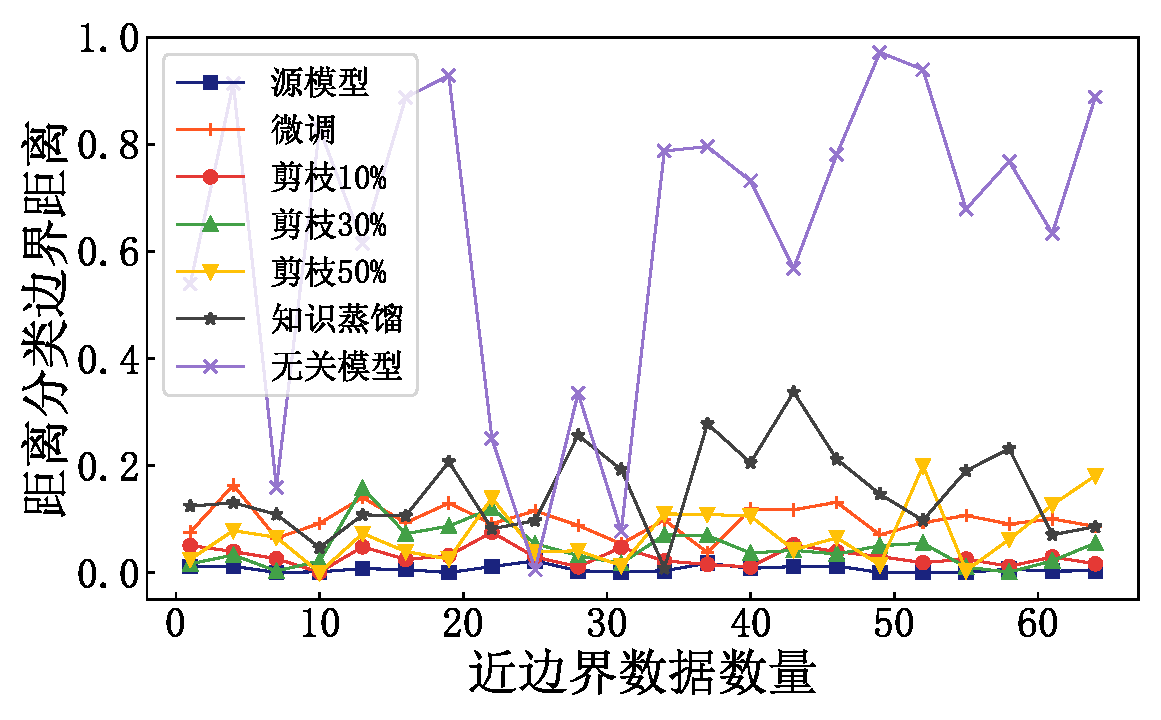
\includegraphics[width=0.49\linewidth]{CIFAR-10-4-3-distance.pdf}}
    \subfigure{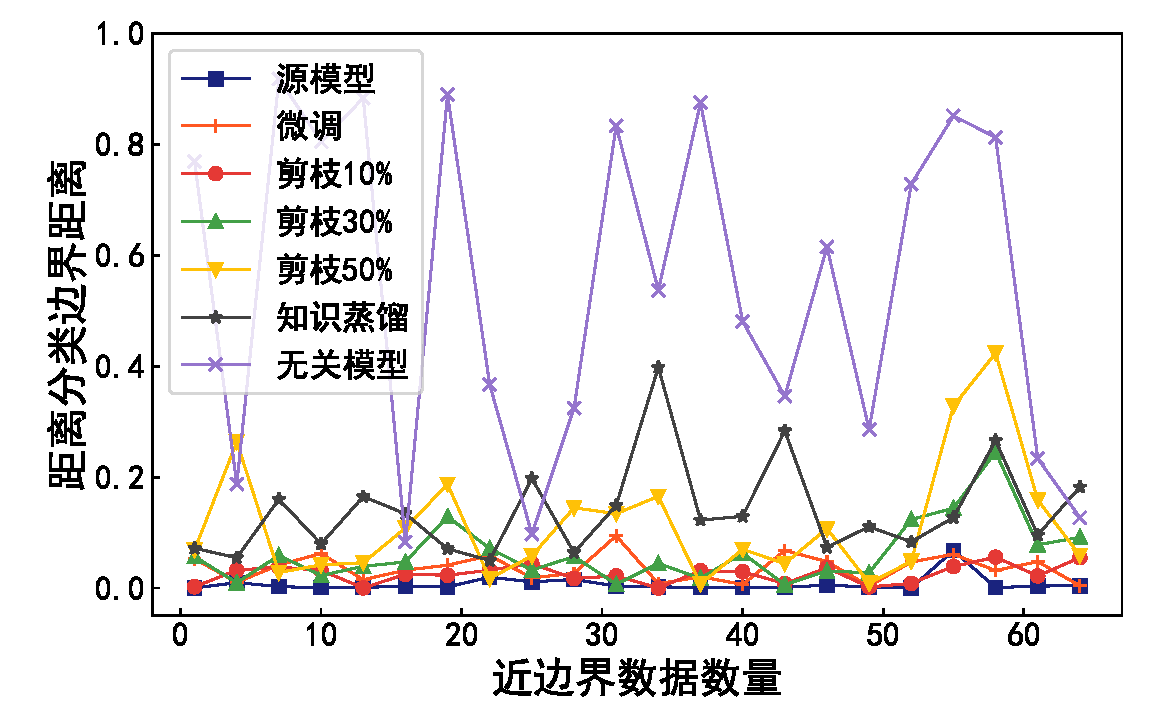
\includegraphics[width=0.49\linewidth]{CIFAR-10-4-7-distance.pdf}}
    \subfigure{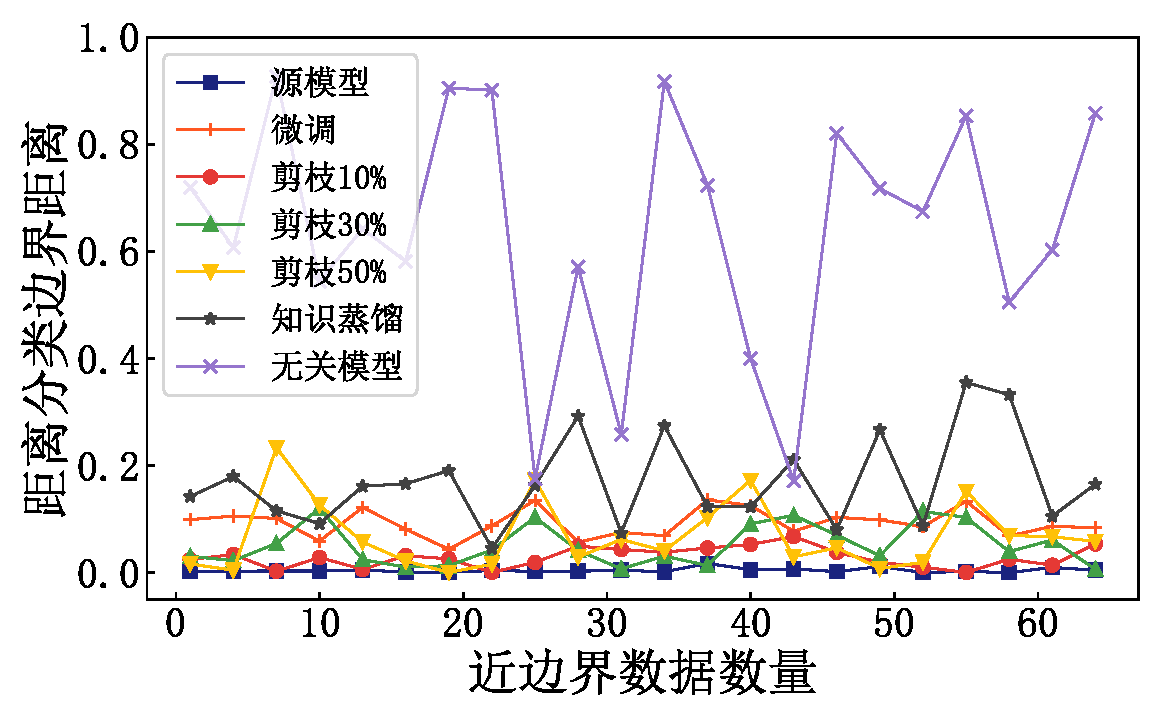
\includegraphics[width=0.49\linewidth]{CIFAR-10-5-6-distance.pdf}}
	\caption{CIFAR-10上4个不同分类边界下的近边界数据表现}
	\label{CIFAR-10上不同分类边界下的近边界数据表现}
\end{figure}

\begin{figure}[!htb]
	\centering
%	\setlength{\abovecaptionskip}{0mm}
%		\vspace{-3mm}
%	\setlength{\belowcaptionskip}{-4mm} %调整图片标题与下文距离
	\subfigure{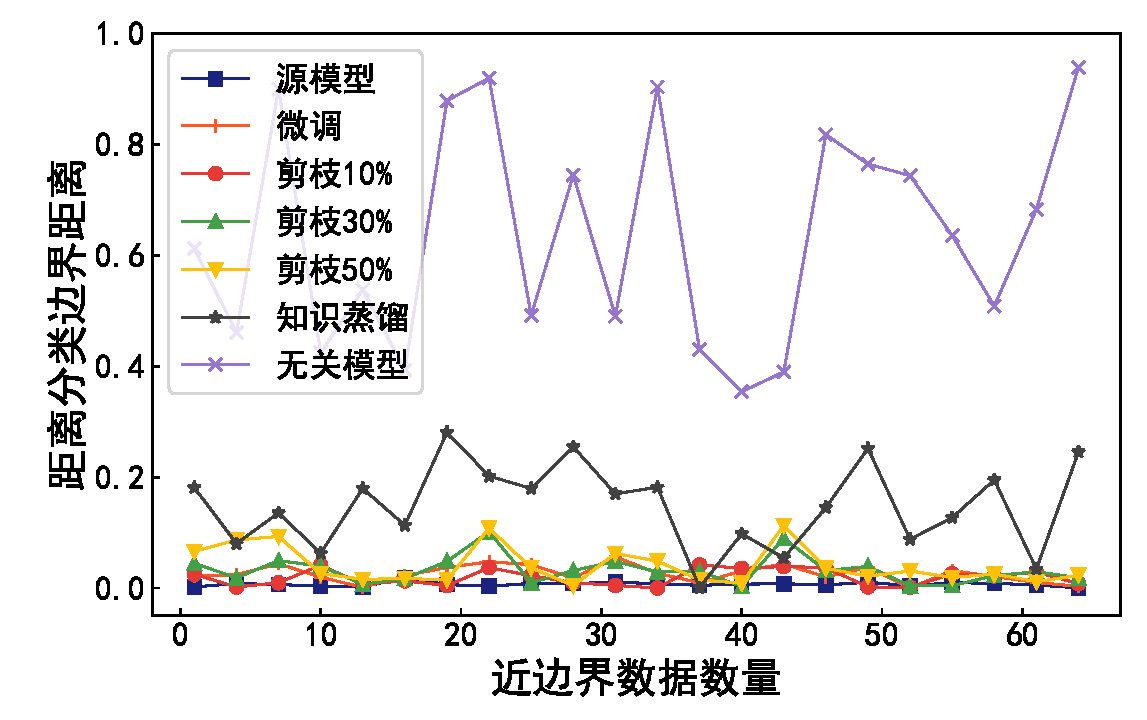
\includegraphics[width=0.49\linewidth]{Heritage-3-0-distance.pdf}} 
	\subfigure{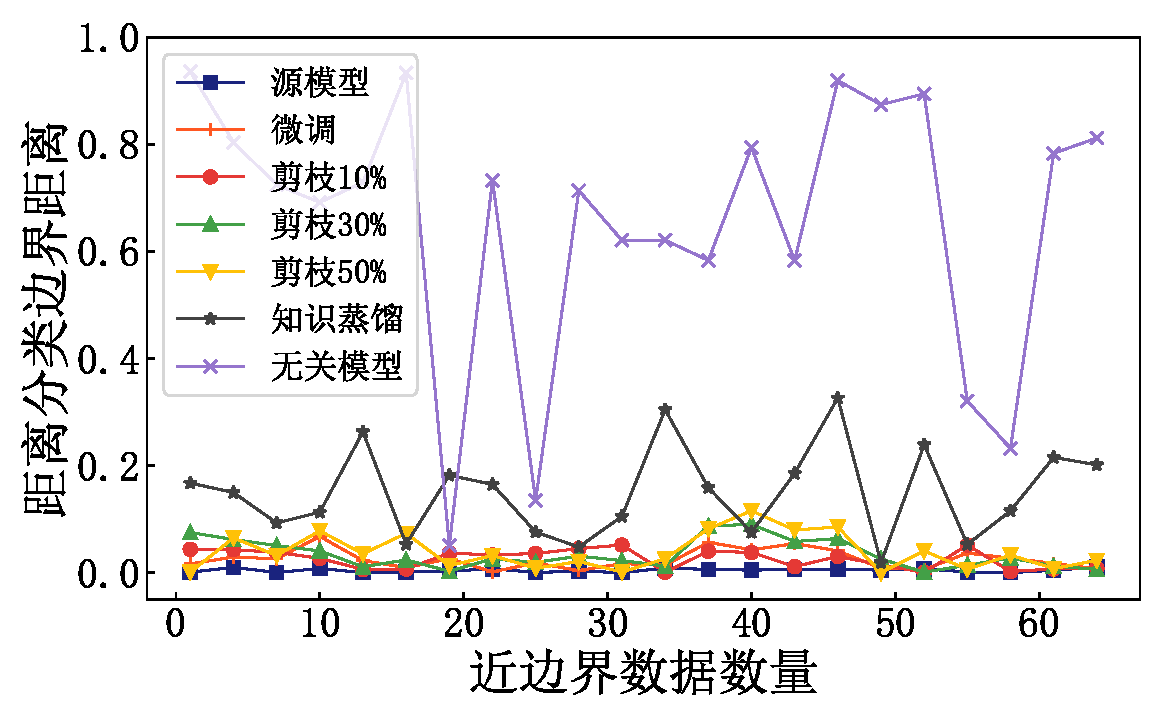
\includegraphics[width=0.49\linewidth]{Heritage-3-1-distance.pdf}} 
	\subfigure{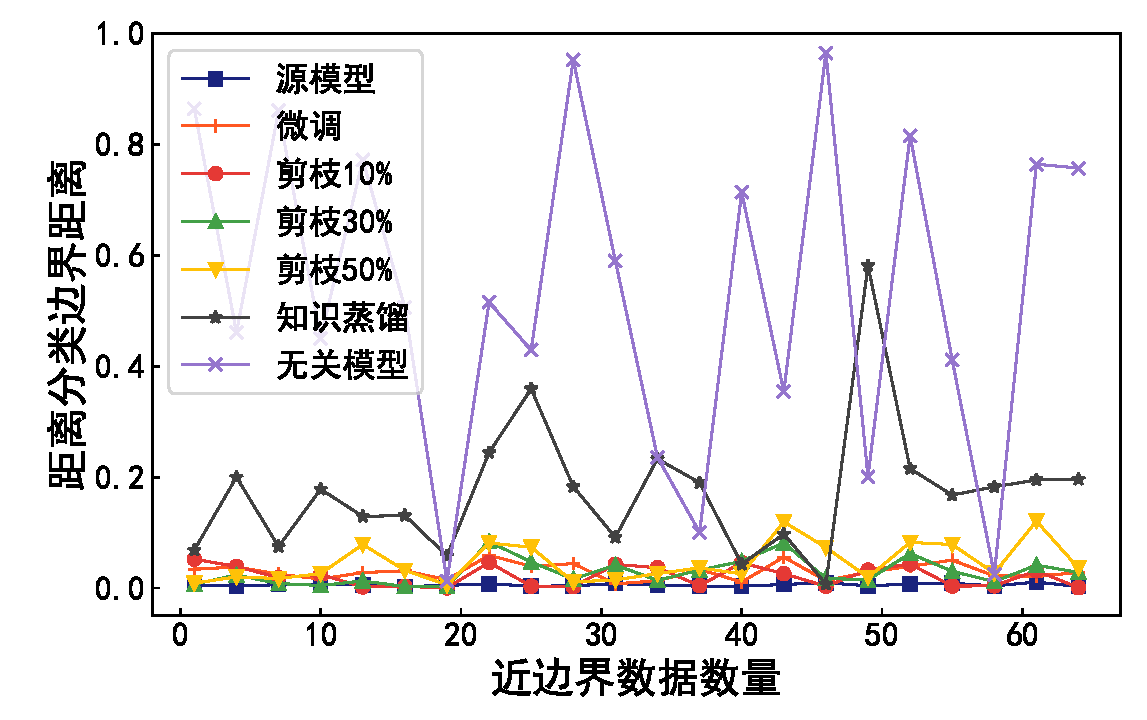
\includegraphics[width=0.49\linewidth]{Heritage-3-4-distance.pdf}} 
	\subfigure{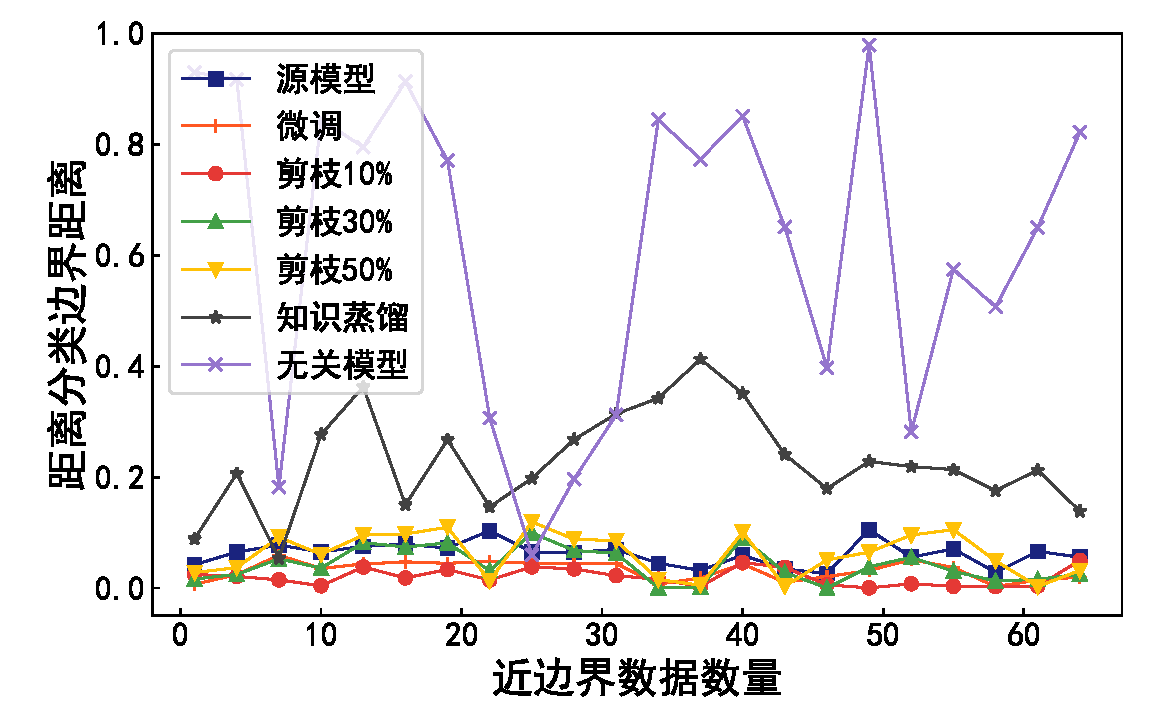
\includegraphics[width=0.49\linewidth]{Heritage-7-6-distance.pdf}} 
	\caption{Heritage上4个不同分类边界下的近边界数据表现}
	\label{Heritage上不同分类边界下的近边界数据表现}
\end{figure}

\begin{figure}[!htb]
	\centering
	\subfigure{\includegraphics[width=0.49\linewidth]{Intel\_image-3-1-distance.pdf}} 
	\subfigure{\includegraphics[width=0.49\linewidth]{Intel\_image-3-4-distance.pdf}} 
	\subfigure{\includegraphics[width=0.49\linewidth]{Intel\_image-3-5-distance.pdf}} 
	\subfigure{\includegraphics[width=0.49\linewidth]{Intel\_image-5-0-distance.pdf}}
	\caption{Intel\_image上4个不同分类边界下的近边界数据表现}
	\label{Intel-image上不同分类边界下的近边界数据表现}
\end{figure}

如图\ref{CIFAR-10上不同分类边界下的近边界数据表现},图\ref{Heritage上不同分类边界下的近边界数据表现},图\ref{Intel-image上不同分类边界下的近边界数据表现}所示, 本文提出的近边界数据在所有盗窃模型中都表现出了靠近分类边界的特性。从图中可以看出,相比于其他所有模型,近边界数据在源模型上距离分类边界的距离最近,这主要是三方面的原因:

1)初始的近边界样本是在源模型的基础上生成的,并且从众多生成对抗性样本的方法中挑选了效果最好的CW-$L_2$方法,然后对该方法进行改进,使之生成距离分类边界更近的对抗性样本。

2)使用DCGAN生成器私有化近边界数据后,设计了新的损失函数微调源模型,这使得私有近边界数据同样非常靠接模型分类边界。

3)被盗模型在从源模型派生的过程中,涉及到模型的修改,这些修改操作虽然不会使近边界数据在这些模型上失去近边界性,但是会使它们稍微偏离模型分类边界。


近边界数据在所有被盗模型中变现出近边界性说明近边界性是可以跟随源模型一起转移的,这跟DNN分类器有很大的关系。对抗性样本一般位于分类边界上,可以反应分类边界,并且这类特殊的样本具有可转移性,近边界数据是利用对抗性样本构造的,同样具有这种特性。这是本文提出方法的重要基础,因为我们就是要利用所有者的私有近边界数据和可疑队友提供的近边界数据到分类边界的距离来推断模型所有权(距离近者获得所有权),如果私有近边界数据不表现出近边界性,那么就会判定失败。

从图中可以发现,相比于其他模型盗窃方法,近边界数据在知识蒸馏派生出的模型上距离分类边界距离稍远。这是因为知识蒸馏对模型的修改特别大,通常来说会更换模型的架构,然后在通过蒸馏的方法训练。模型知识蒸馏对于其他模型知识产权保护方法也是一种挑战,近边界数据在蒸馏产生的模型上仍然表现出近边界性,因此本文提出的方法对这种强修改的盗窃方法依然适用。

图中还有一个点是近边界数据在无关模型上并不反映出近边界性,这是非常重要的。本文提出的方法不应该对正常的无关模型产生误判,混淆所有权的归属。

在这一阶段,我们使用的近边界数据大小为64。也就是说,本文的方法在较小规模近边界数据时效果依然显著,那么在增大数据量时,效果会更加明显。在\ref{5.6}中,我们会对不同规模的近边界数据进行测试。

\section{微调目标分类边界的影响}\label{5.4}

本小节将对\ref{3}\ref{3.3}中使用私有近边界数据微调源模型产生的影响进行测试。我们针对不同数据集训练得到的源模型,使用不同规模的近边界数据以及不同的目标分类边界对源模型进行微调。
\begin{table}[h]
	\centering
	%	\setlength{\arrayrulewidth}{0.5mm}
	\renewcommand\arraystretch{1.2}
	\caption{微调分类边界对准确率的影响}
	\label{table:3}
	\resizebox{\linewidth}{!}{
	\begin{tabular}{l c c c c}
		\hline
		\multirow{3}{5em}{分类边界}&\multirow{3}{5em}{数据大小} & CIFAR-10&Heritage&Intel\_image \\ 
		& & 准确率(0.886)&准确率(0.879)&准确率(0.854) \\
		\cline{3-5}	
		& &准确率&准确率&准确率 \\
		\hline
		\multirow{4}{5em}{分类边界1}&64&0.873&0.862&0.825 \\
		&128&0.862&0.858&0.829 \\
		&256&0.862&0.854&0.826 \\
		&512&0.856&0.848&0.839 \\
		\hline
		\multirow{4}{5em}{分类边界2}&64&0.871&0.867&0.843 \\
		&128&0.870&0.862&0.839 \\
		&256&0.860&0.859&0.828 \\
		&512&0.859&0.851&0.824 \\
		\hline
		\multirow{4}{5em}{分类边界3}&64&0.871&0.865&0.841 \\
		&128&0.868&0.857&0.833 \\
		&256&0.858&0.855&0.831 \\
		&512&0.855&0.851&0.823 \\
		\hline
		\multirow{4}{5em}{分类边界4}&64&0.873&0.863&0.847 \\
		&128&0.873&0.860&0.843 \\
		&256&0.866&0.854&0.838 \\
		&512&0.862&0.849&0.831 \\
		\hline
		\multirow{4}{5em}{分类边界5}&64&0.876&0.866&0.846 \\
		&128&0.866&0.861&0.834 \\
		&256&0.868&0.857&0.829 \\
		&512&0.861&0.853&0.825 \\
		\hline
\end{tabular}
}
\end{table}

	
如表\ref{table:3}所示,随着微调模型近边界数量的增多,模型准确率逐渐下降,但是在几乎全部情况下,源模型微调前后的精度差没有超过3\%,这是本文方法可以接受的范围。因为私有近边界数据本身不是原始数据集的一部分,所以使用规模变大时,对源模型的影响也会变大。但是在另一个角度,微调源模型的目的是使得我们的私有近边界数据更加靠近分类边界,来提高后续推断模型所有权的置信度,所以,使用更多的近边界数据微调源模型效果会更好。因此,在实际情况中,微调数据规模的选择是一个模型精度和推断置信度的折衷。

表中整体情况下,模型的准确率都下降不多。一方面,这是因为本身微调的数据和源模型的训练数据相比只是一小部分,不会对模型产生太大的影响。另一方面,在微调源模型时,我们将学习率设置为0.0001,这是很低的。并且使用原始数据对模型进行交替训练,训练轮次不超过10次。所以微调之后,模型准确率没有受到很大的影响。

实验结果证明,本文的私有近边界数据在应用于模型所有权保护问题时,模型具有较好的保真度。因此,使用近边界数据推断模型所有权不用担心源模型受到较大的影响。	
	

\section{推断模型所有权的有效性}\label{5.5}

本文提出的方法目的是推断模型所有权,本节将对此方法的有效性进行测试。根据本文提出方法的流程,模型所有者和可疑对手均需要提供各自的近边界数据,然后输入模型获得输出,再根据\ref{4.2.3}中提到的假设检验进行结果比对,判断可疑模型是否从源模型派生。

\begin{table}[h]
	\centering
%	\setlength{\arrayrulewidth}{0.5mm}
	\renewcommand\arraystretch{1.5}
	\caption{推断模型所有权}
	\label{table:2}
	\resizebox{\linewidth}{!}{
	\begin{tabular}{l l c c c c c c c c c c}
		
		\hline
\multirow{2}{5em}{数据集}&\multirow{2}{4em}{攻击方法}&\multicolumn{2}{c}{分类边界1}&\multicolumn{2}{c}{分类边界2}&\multicolumn{2}{c}{分类边界3}&\multicolumn{2}{c}{分类边界4}&\multicolumn{2}{c}{分类边界5}\\ \cline{3-12}
		                         & &$\Delta\mu$&$p$值&$\Delta\mu$&$p$值&$\Delta\mu$&$p$值&$\Delta\mu$&$p$值&$\Delta\mu$&$p$值 \\
		\hline
\multirow{6}{5em}{CIFAR-10}     &源模型    & 0.913 & $10^{-6}$ & 0.954 & $10^{-6}$ & 0.927 & $10^{-5}$ & 0.967 & $10^{-5}$ & 0.958 & $10^{-5}$   \\
								&模型微调  & 0.718 & $10^{-5}$ & 0.745 & $10^{-6}$ & 0.698 & $10^{-5}$ & 0.692 & $10^{-4}$ & 0.729 & $10^{-5}$   \\
								& 剪枝10\% & 0.572 & $10^{-5}$ & 0.487 & $10^{-5}$ & 0.458 & $10^{-5}$ & 0.533 & $10^{-4}$ & 0.512 & $10^{-4}$   \\
								&剪枝30\%  & 0.537 & $10^{-4}$ & 0.497 & $10^{-4}$ & 0.401 & $10^{-3}$ & 0.428 & $10^{-4}$ & 0.587 & $10^{-4}$   \\
								&剪枝50\%  & 0.545 & $10^{-4}$ & 0.614 & $10^{-4}$ & 0.506 & $10^{-3}$ & 0.570 & $10^{-4}$ & 0.484 & $10^{-3}$   \\
								&知识蒸馏  & 0.372 & $10^{-3}$ & 0.297 & $10^{-3}$ & 0.288 & $10^{-3}$ & 0.308 & $10^{-3}$ & 0.340 & $10^{-3}$   \\
		\hline
\multirow{6}{5em}{Heritage}     &源模型    & 0.876 & $10^{-5}$ & 0.845 & $10^{-5}$ & 0.859 & $10^{-4}$ & 0.801 & $10^{-4}$ & 0.837 & $10^{-5}$   \\
								&模型微调  & 0.815 & $10^{-5}$ & 0.792 & $10^{-4}$ & 0.824 & $10^{-4}$ & 0.833 & $10^{-4}$ & 0.784 & $10^{-4}$   \\
								&剪枝10\%  & 0.530 & $10^{-4}$ & 0.535 & $10^{-3}$ & 0.508 & $10^{-4}$ & 0.486 & $10^{-3}$ & 0.471 & $10^{-3}$   \\
								&剪枝30\%  & 0.491 & $10^{-3}$ & 0.452 & $10^{-3}$ & 0.469 & $10^{-4}$ & 0.470 & $10^{-3}$ & 0.427 & $10^{-4}$   \\
								&剪枝50\%  & 0.502 & $10^{-3}$ & 0.517 & $10^{-3}$ & 0.434 & $10^{-3}$ & 0.451 & $10^{-3}$ & 0.490 & $10^{-3}$   \\
								&知识蒸馏  & 0.329 & $10^{-3}$ & 0.365 & $10^{-2}$ & 0.238 & $10^{-3}$ & 0.310 & $10^{-3}$ & 0.274 & $10^{-3}$   \\
		\hline
\multirow{6}{5em}{Intel\_image} &源模型    & 0.859 & $10^{-5}$ & 0.896 & $10^{-4}$ & 0.872 & $10^{-4}$ & 0.899 & $10^{-4}$ & 0.914 & $10^{-4}$   \\
								&模型微调  & 0.717 & $10^{-5}$ & 0.784 & $10^{-4}$ & 0.752 & $10^{-4}$ & 0.791 & $10^{-3}$ & 0.709 & $10^{-4}$   \\
								&剪枝10\%  & 0.451 & $10^{-4}$ & 0.522 & $10^{-4}$ & 0.539 & $10^{-3}$ & 0.472 & $10^{-3}$ & 0.438 & $10^{-4}$   \\
								&剪枝30\%  & 0.407 & $10^{-4}$ & 0.415 & $10^{-4}$ & 0.346 & $10^{-3}$ & 0.382 & $10^{-3}$ & 0.395 & $10^{-3}$   \\
								&剪枝50\%  & 0.370 & $10^{-3}$ & 0.395 & $10^{-3}$ & 0.327 & $10^{-3}$ & 0.360 & $10^{-3}$ & 0.458 & $10^{-3}$   \\
								&知识蒸馏  & 0.336 & $10^{-2}$ & 0.395 & $10^{-3}$ & 0.360 & $10^{-2}$ & 0.308 & $10^{-3}$ & 0.287 & $10^{-2}$   \\
		\hline		
	\end{tabular}
}
\end{table}

在本节中,我们讨论本文方法生成的私有近边界数据与其他近边界数据在盗窃模型上的性能对比。首先,我们模拟了盗窃者可能会提供的近边界数据,该数据由两部分组成,包括(1)从原始数据中挑选出的近边界数据,(2)由FGSM和CW生成的一些对抗性样本。然后针对不同的目标分类边界,进行假设检验并计算在不同数据集和不同盗窃模型上的$\Delta\mu$和$p$值。

如表\ref{table:2}所示,$p$值在每个数据集,每条分类边界上呈从上到下增大的趋势,$\Delta\mu$呈减小趋势,在全部情况中,$p$值均低于0.05。
也就是说,本文的方法在不同的盗窃方法中推断模型的所有权均有显著的效果,我们至少有95\%以上的置信度确定可疑模型是盗窃模型。

在假设检验中,$p$值越小,$\Delta\mu$越大说明结果越可靠,推断的置信度越高。表中从上到小$p$值减小是因为这些方法对模型的修改逐渐增大,尤其是在知识蒸馏上,模型知识蒸馏是本文方法的最大挑战,也同样是其他研究面临的巨大挑战。在我们的实验中,可以观察到我们的方法始终可以将蒸馏模型推断为被盗模型。因此,实验结果表明使用私有的近边界数据对大多数模型盗窃技术都是可靠的,我们可以声称模型被盗窃的置信度至少为95\%,证明了本文方法的有效性和鲁棒性。


\section{不同规模近边界数据的可伸缩性扩展}\label{5.6}

在本节中,我们将测试不同规模的近边界数据在推断模型所有权上的可伸缩性。我们的方法需要对数据进行采样从而进行假设检验,通常来说样本数量越大,对检验过程中因随机因素而产生的不利影响就会越小,更能准确的推断模型所有权。

\begin{figure}[!htb]
	\centering
	\subfigure{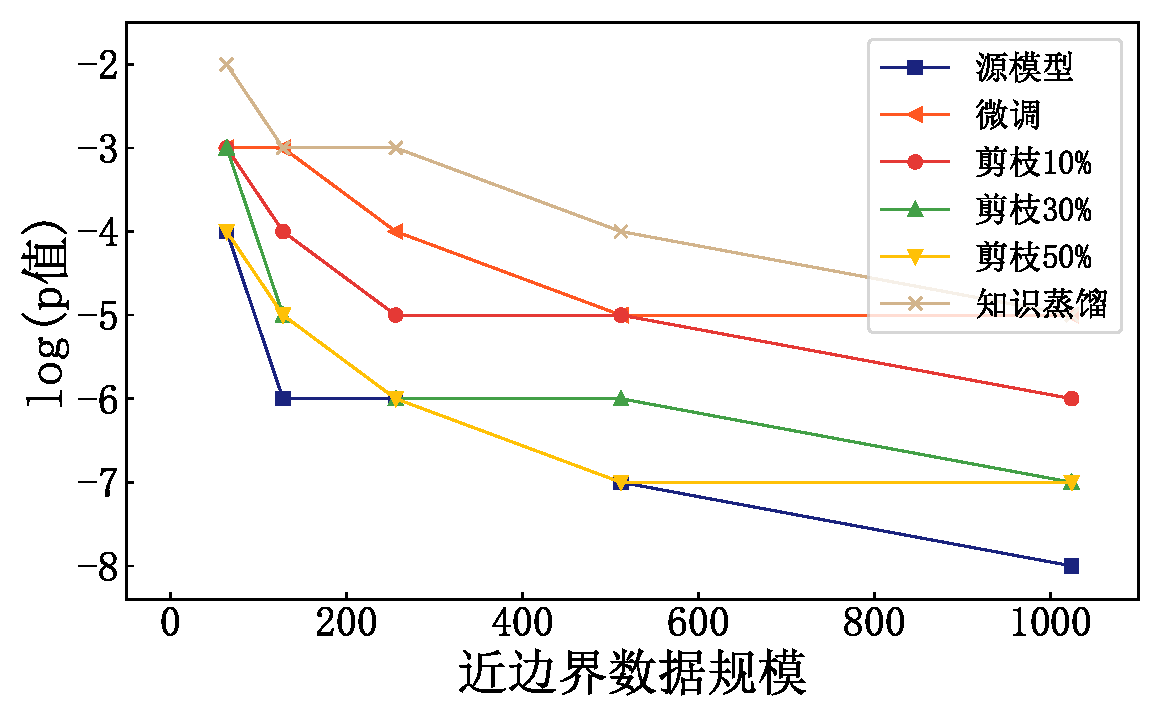
\includegraphics[width=0.49\linewidth]{CIFAR-10-4-2-p-value.pdf}} 
	\subfigure{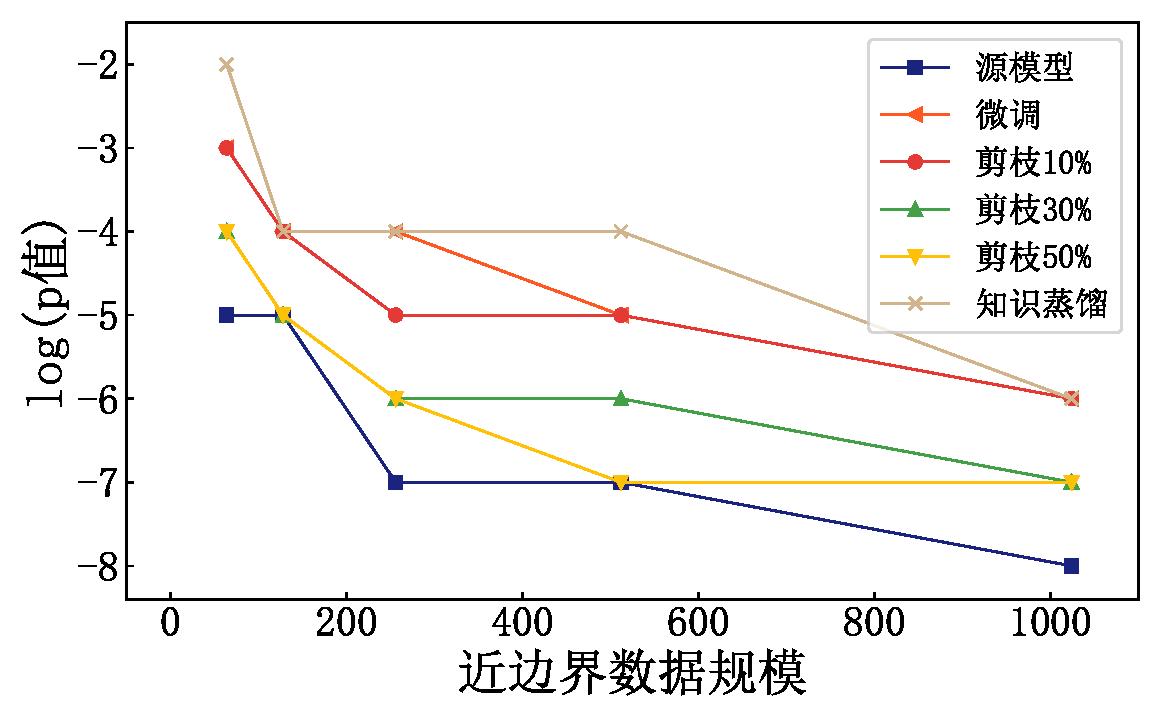
\includegraphics[width=0.49\linewidth]{CIFAR-10-4-3-p-value.pdf}}
	\subfigure{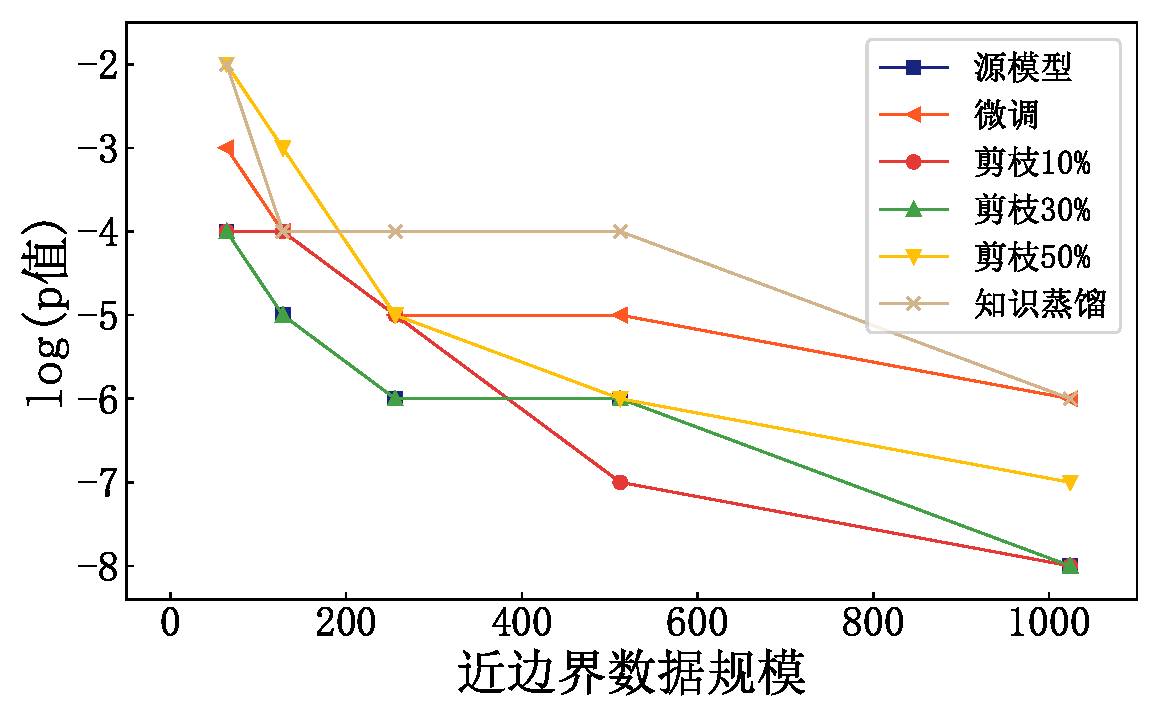
\includegraphics[width=0.49\linewidth]{CIFAR-10-4-7-p-value.pdf}}
	\subfigure{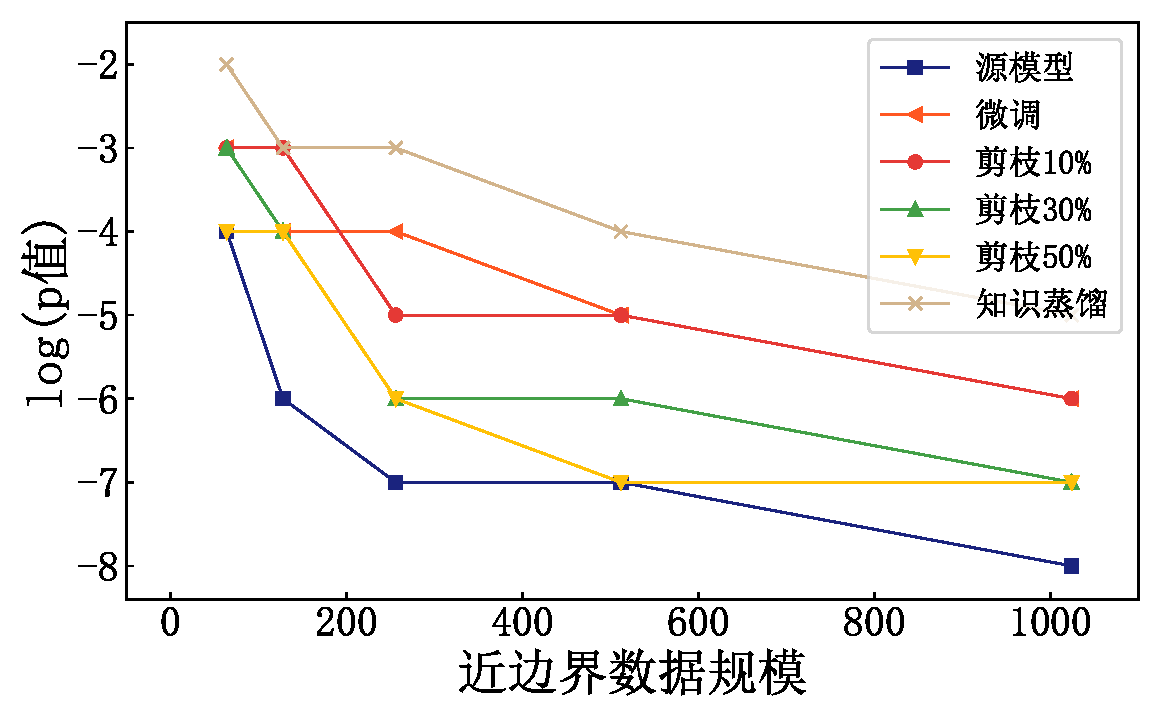
\includegraphics[width=0.49\linewidth]{CIFAR-10-5-6-p-value.pdf}} 
	\caption{CIFAR-10上4个不同分类边界下的扩展}
	\label{CIFAR-10上推断模型所有权的扩展性}
%	\setlength{\abovecaptionskip}{7mm}
\end{figure}

\begin{figure}[!htb]
	\centering
	\subfigure{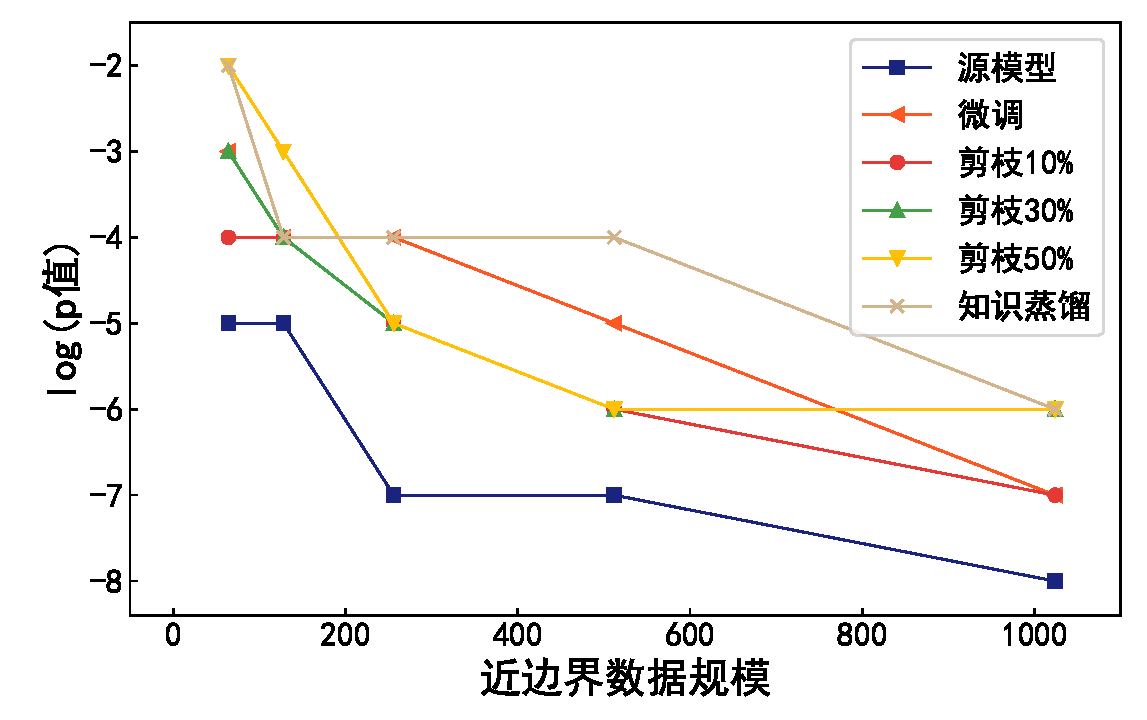
\includegraphics[width=0.49\linewidth]{Heritage-3-0-p-value.pdf}} 
	\subfigure{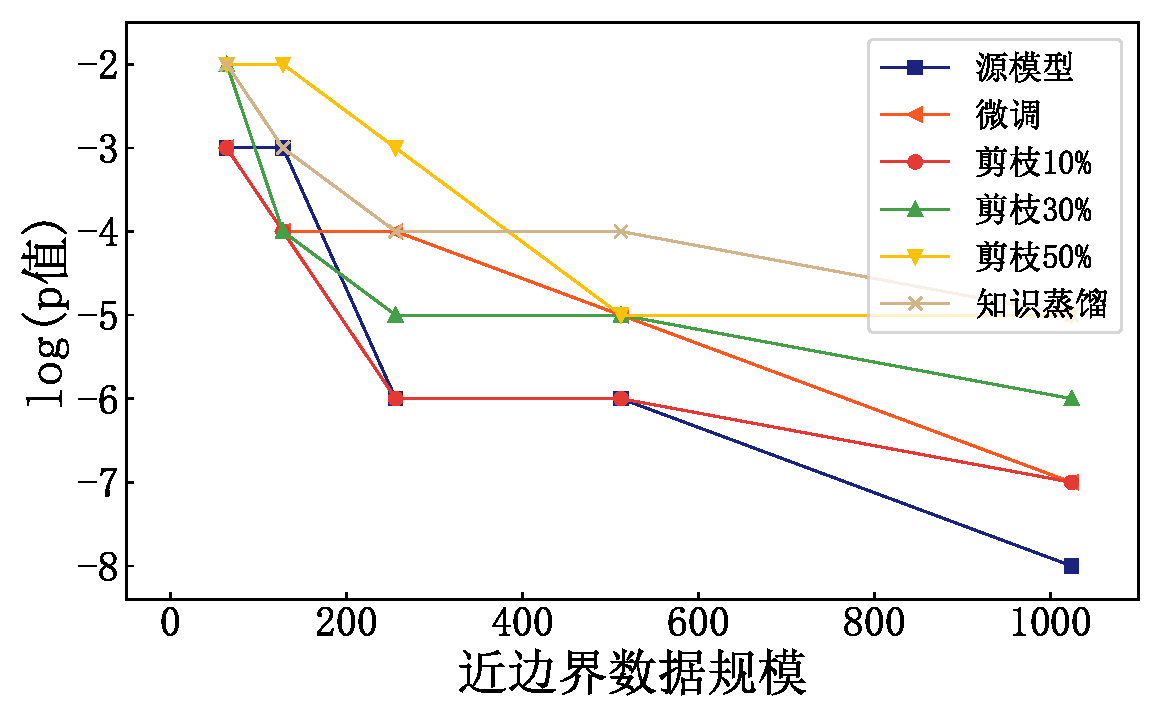
\includegraphics[width=0.49\linewidth]{Heritage-3-1-p-value.pdf}} 
	\subfigure{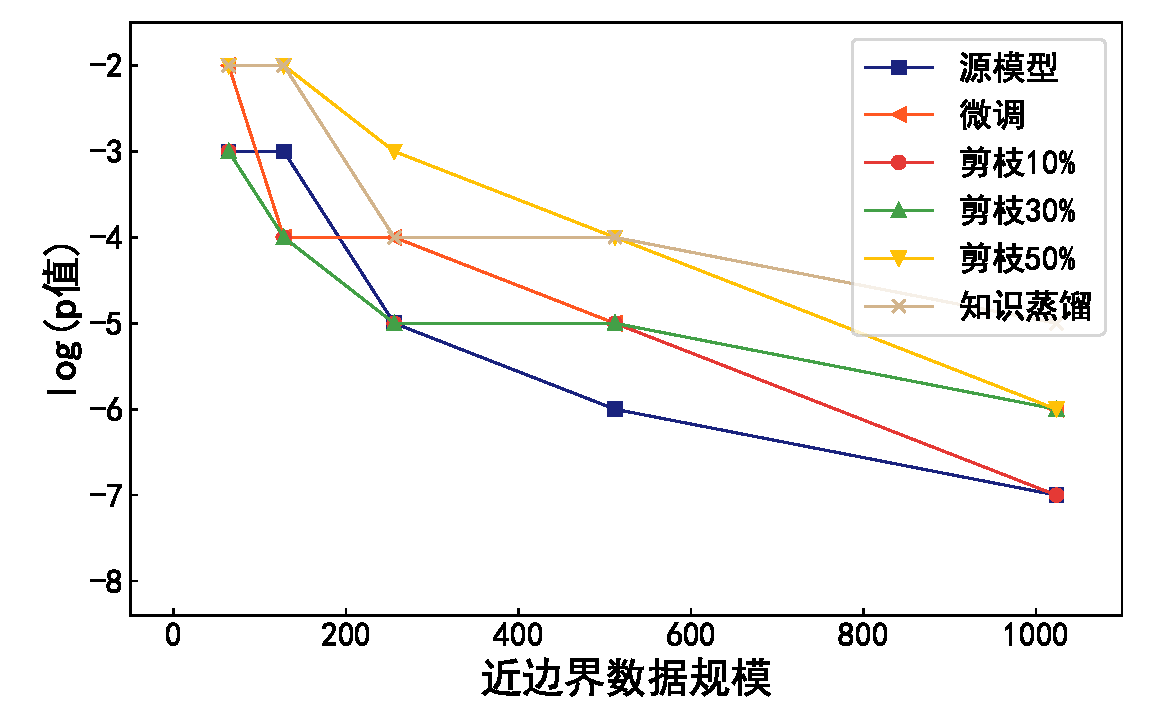
\includegraphics[width=0.49\linewidth]{Heritage-3-4-p-value.pdf}} 
	\subfigure{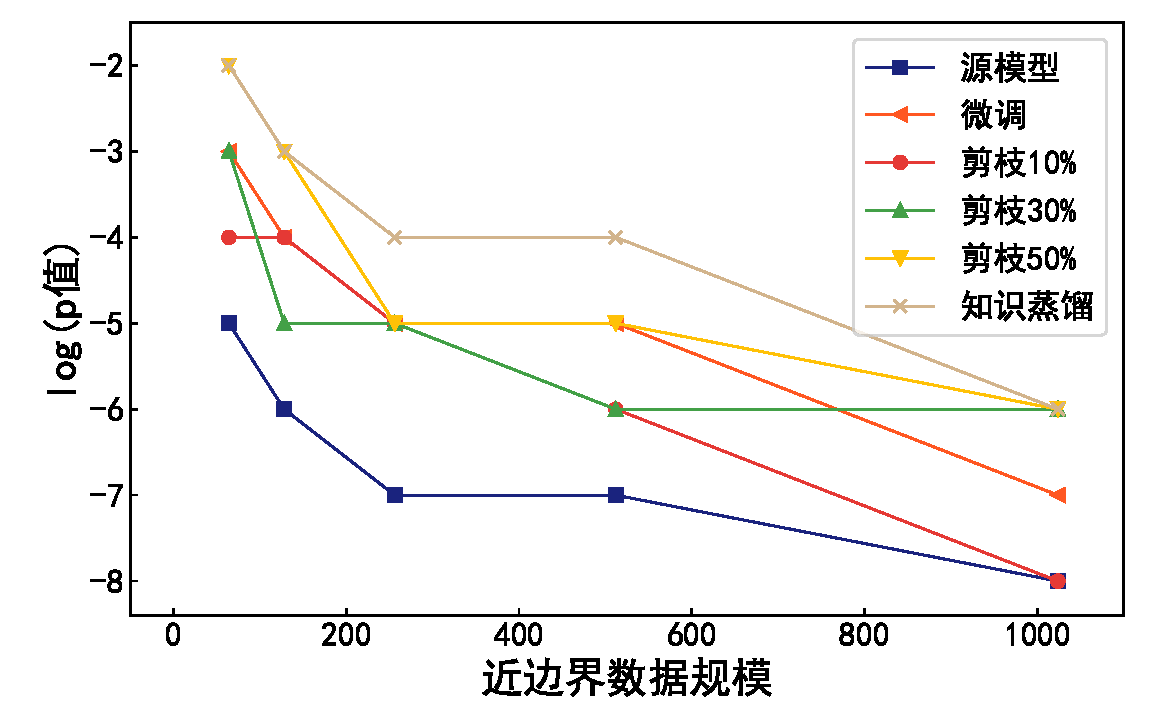
\includegraphics[width=0.49\linewidth]{Heritage-7-6-p-value.pdf}} 
	\caption{Heritage上4个不同分类边界下的扩展}
	\label{Heritage上推断模型所有权的扩展性}
%	\setlength{\abovecaptionskip}{7mm}
\end{figure}

\begin{figure}[!htb]
	\centering
	\subfigure{\includegraphics[width=0.49\linewidth]{Intel\_image-3-1-p-value.pdf}} 
	\subfigure{\includegraphics[width=0.49\linewidth]{Intel\_image-3-4-p-value.pdf}} 
	\subfigure{\includegraphics[width=0.49\linewidth]{Intel\_image-3-5-p-value.pdf}} 
	\subfigure{\includegraphics[width=0.49\linewidth]{Intel\_image-5-0-p-value.pdf}} 
	\caption{Intel\_image上4个不同分类边界下的扩展}
	\label{Intel-image上推断模型所有权的扩展性}
%	\setlength{\abovecaptionskip}{7mm}
\end{figure}

如图\ref{CIFAR-10上推断模型所有权的扩展性},图\ref{Heritage上推断模型所有权的扩展性},图\ref{Intel-image上推断模型所有权的扩展性}所示,$p$值在不同数据集,不同分类边界上,随着近边界数据规模的增大而减小,而$p$值越小说明假设检验能够以更高的置信度确定可疑模型是被盗模型。

本文的方法在进行假设检验前,需要将私有的近边界数据和可疑对手的近边界数据分别输入可疑模型。可疑对手近边界数据是通过从原始数据挑选和FGSM,CW生成的对抗性样本组成的。因此,由于随机因素,存在一小部分可疑对手的数据到分类边界的距离和我们的私有近边界数据相近,甚至比我们的小,这会导致一定的误判情况。随着测试样本的增大,这种随机因素的影响会被逐渐消除,所以从图中可以观察到,随着近边界数据规模的增大,$p$值逐渐减小。但这并不说明我们的方法对小数量的近边界数据缺少鲁棒性,从图中我们可以观察到即使数据量为64的情况下,$p$值仍然小于0.05,这证明我们的方法对于小数样本量同样有显著的效果。

\section{本章小结}

本章我们在CIFAR-10,Heritage,Intel\_image这三个数据集上对本文提出的方法进行了全面的测评分析。首先对各种对抗性样本生成方法进行测试,初始近边界数据生成算法的选择非常重要,这影响到生成数据到分类边界的距离,是方法最后假设检验的指标。接着对数据近边界特性进行了评估,结果表明近边界数据的近边界性可以从源模型转移到派生出的模型上,这是本文方法的重要基础。然后测试了微调分类边界对模型准确率的影响,因为本文的方法不应该对模型精度造成很大的影响,否则该方法失去了意义。接着测试了本文方法推断模型所有权的有效性,结果表明该方法对不同的模型盗窃方法均能以95\%以上的置信度声明可疑模型是盗窃模型。最后对假设检验样本规模进行了扩展,在更大规模的情况下,本文的方法会更加有效,当然,也适用于类似64的小样本数据情况。

